\documentclass[12pt]{article}
\usepackage{amsmath}
\usepackage{amssymb}
\usepackage{geometry}
\usepackage{enumerate}
\usepackage{natbib}
\usepackage{float}%稳定图片位置
\usepackage{graphicx}%画图
\usepackage[english]{babel}
\usepackage{a4wide}
\usepackage{indentfirst}%缩进
\usepackage{enumerate}%加序号
\usepackage{multirow}%合并行
\title{\large UM-SJTU JOINT INSTITUTE\\Advanced Lasers and Optics Laboratory\\(VE438)\\\ \\\ \\\ \\\ \\\ \\\ \\\ \\\ \\\ \\\ \\\
Pre Lab Assignment\\\ \\\ LAB 5\\\ Spectrometer \\\ \\\ \\\ \\\ \\\ }
\author{Name: Pan Chongdan \\ID: 516370910121}
\date{Date: \today}

\begin{document}
\maketitle
\newpage
\section{Answers for Pre Lab Questions}
\subsection{Question 1}
\begin{figure}[H]
\centering
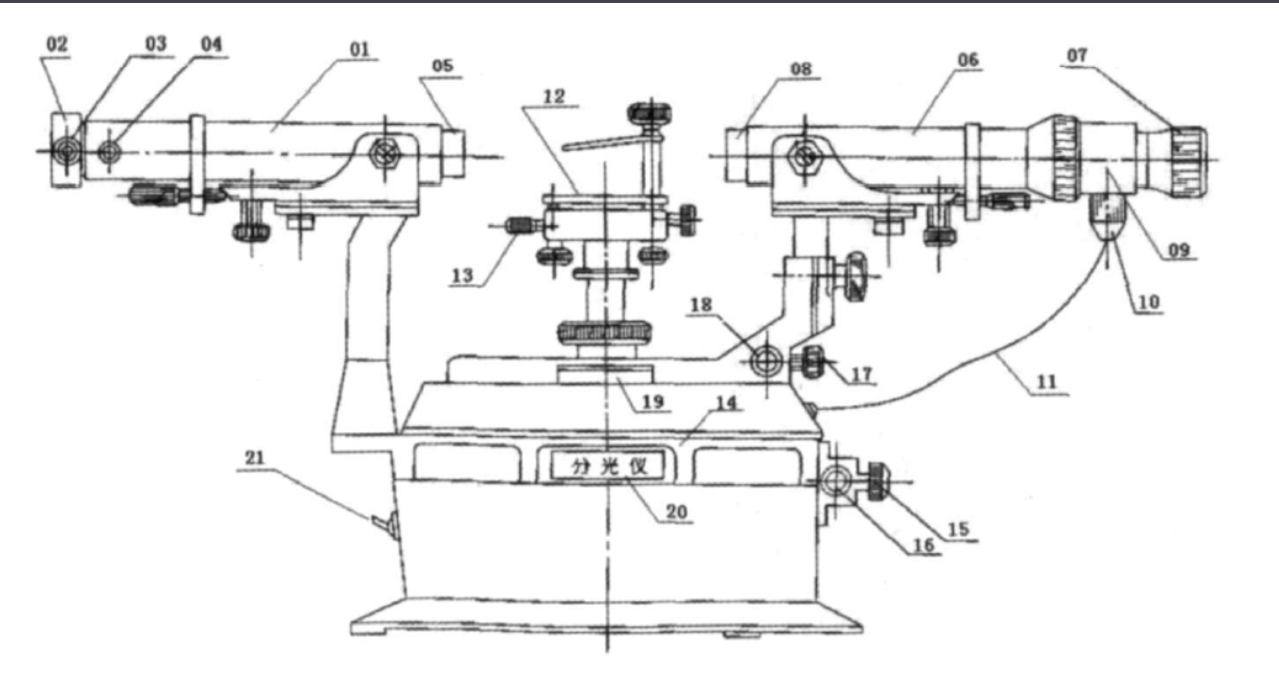
\includegraphics[scale=0.3]{P1.png}
\end{figure}
The is a schematic spectrometer called FGY-01. The light can pass into the spectrometer through part 2, which is a slit. Part 1 is the parallel collimator, which can product parallel light after it pass through the slit.Part 6 and part 8 are lens that can have the parallel focused on part 11 is reticle with a rectangle prism which can produce light of different color by dispersion effect. Then we can observe the result from part 7. User can also put other things on the rest parts to observe their behaviour.
\subsection{Question 2}
The periodicity of grating is the distance between the places where the refractive index has one change and another change. The smaller the period of the grating is smaller, light will form a different patter at a high frequency, which means the spreading angle is smaller.
\par The parallel light produced from collimator can have diffraction through the grating. The relationship can be expressed as $d(\sin\theta\pm\sin i)=m\lambda$ where $i$ is the incident angle and $\theta$ is the diffraction angle, $m$ is the order and $d$ is the period. 
\subsection{Question 3}
For zero-mode grating, according to the equation above, all the diffraction angles for light of different color are same and they can't be split up so we should use the first-order grating so that there is diffraction patterns can be separated.
\end{document}